% Options for packages loaded elsewhere
\PassOptionsToPackage{unicode}{hyperref}
\PassOptionsToPackage{hyphens}{url}
\PassOptionsToPackage{dvipsnames,svgnames,x11names}{xcolor}
%
\documentclass[
  12pt,
  a4paper,
]{article}
\usepackage{amsmath,amssymb}
\usepackage{lmodern}
\usepackage{setspace}
\usepackage{iftex}
\ifPDFTeX
  \usepackage[T1]{fontenc}
  \usepackage[utf8]{inputenc}
  \usepackage{textcomp} % provide euro and other symbols
\else % if luatex or xetex
  \usepackage{unicode-math}
  \defaultfontfeatures{Scale=MatchLowercase}
  \defaultfontfeatures[\rmfamily]{Ligatures=TeX,Scale=1}
\fi
% Use upquote if available, for straight quotes in verbatim environments
\IfFileExists{upquote.sty}{\usepackage{upquote}}{}
\IfFileExists{microtype.sty}{% use microtype if available
  \usepackage[]{microtype}
  \UseMicrotypeSet[protrusion]{basicmath} % disable protrusion for tt fonts
}{}
\makeatletter
\@ifundefined{KOMAClassName}{% if non-KOMA class
  \IfFileExists{parskip.sty}{%
    \usepackage{parskip}
  }{% else
    \setlength{\parindent}{0pt}
    \setlength{\parskip}{6pt plus 2pt minus 1pt}}
}{% if KOMA class
  \KOMAoptions{parskip=half}}
\makeatother
\usepackage{xcolor}
\usepackage[left=2.54cm,right=2.54cm,top=2.54cm,bottom=2.54cm]{geometry}
\usepackage{color}
\usepackage{fancyvrb}
\newcommand{\VerbBar}{|}
\newcommand{\VERB}{\Verb[commandchars=\\\{\}]}
\DefineVerbatimEnvironment{Highlighting}{Verbatim}{commandchars=\\\{\}}
% Add ',fontsize=\small' for more characters per line
\usepackage{framed}
\definecolor{shadecolor}{RGB}{248,248,248}
\newenvironment{Shaded}{\begin{snugshade}}{\end{snugshade}}
\newcommand{\AlertTok}[1]{\textcolor[rgb]{0.94,0.16,0.16}{#1}}
\newcommand{\AnnotationTok}[1]{\textcolor[rgb]{0.56,0.35,0.01}{\textbf{\textit{#1}}}}
\newcommand{\AttributeTok}[1]{\textcolor[rgb]{0.77,0.63,0.00}{#1}}
\newcommand{\BaseNTok}[1]{\textcolor[rgb]{0.00,0.00,0.81}{#1}}
\newcommand{\BuiltInTok}[1]{#1}
\newcommand{\CharTok}[1]{\textcolor[rgb]{0.31,0.60,0.02}{#1}}
\newcommand{\CommentTok}[1]{\textcolor[rgb]{0.56,0.35,0.01}{\textit{#1}}}
\newcommand{\CommentVarTok}[1]{\textcolor[rgb]{0.56,0.35,0.01}{\textbf{\textit{#1}}}}
\newcommand{\ConstantTok}[1]{\textcolor[rgb]{0.00,0.00,0.00}{#1}}
\newcommand{\ControlFlowTok}[1]{\textcolor[rgb]{0.13,0.29,0.53}{\textbf{#1}}}
\newcommand{\DataTypeTok}[1]{\textcolor[rgb]{0.13,0.29,0.53}{#1}}
\newcommand{\DecValTok}[1]{\textcolor[rgb]{0.00,0.00,0.81}{#1}}
\newcommand{\DocumentationTok}[1]{\textcolor[rgb]{0.56,0.35,0.01}{\textbf{\textit{#1}}}}
\newcommand{\ErrorTok}[1]{\textcolor[rgb]{0.64,0.00,0.00}{\textbf{#1}}}
\newcommand{\ExtensionTok}[1]{#1}
\newcommand{\FloatTok}[1]{\textcolor[rgb]{0.00,0.00,0.81}{#1}}
\newcommand{\FunctionTok}[1]{\textcolor[rgb]{0.00,0.00,0.00}{#1}}
\newcommand{\ImportTok}[1]{#1}
\newcommand{\InformationTok}[1]{\textcolor[rgb]{0.56,0.35,0.01}{\textbf{\textit{#1}}}}
\newcommand{\KeywordTok}[1]{\textcolor[rgb]{0.13,0.29,0.53}{\textbf{#1}}}
\newcommand{\NormalTok}[1]{#1}
\newcommand{\OperatorTok}[1]{\textcolor[rgb]{0.81,0.36,0.00}{\textbf{#1}}}
\newcommand{\OtherTok}[1]{\textcolor[rgb]{0.56,0.35,0.01}{#1}}
\newcommand{\PreprocessorTok}[1]{\textcolor[rgb]{0.56,0.35,0.01}{\textit{#1}}}
\newcommand{\RegionMarkerTok}[1]{#1}
\newcommand{\SpecialCharTok}[1]{\textcolor[rgb]{0.00,0.00,0.00}{#1}}
\newcommand{\SpecialStringTok}[1]{\textcolor[rgb]{0.31,0.60,0.02}{#1}}
\newcommand{\StringTok}[1]{\textcolor[rgb]{0.31,0.60,0.02}{#1}}
\newcommand{\VariableTok}[1]{\textcolor[rgb]{0.00,0.00,0.00}{#1}}
\newcommand{\VerbatimStringTok}[1]{\textcolor[rgb]{0.31,0.60,0.02}{#1}}
\newcommand{\WarningTok}[1]{\textcolor[rgb]{0.56,0.35,0.01}{\textbf{\textit{#1}}}}
\usepackage{longtable,booktabs,array}
\usepackage{calc} % for calculating minipage widths
% Correct order of tables after \paragraph or \subparagraph
\usepackage{etoolbox}
\makeatletter
\patchcmd\longtable{\par}{\if@noskipsec\mbox{}\fi\par}{}{}
\makeatother
% Allow footnotes in longtable head/foot
\IfFileExists{footnotehyper.sty}{\usepackage{footnotehyper}}{\usepackage{footnote}}
\makesavenoteenv{longtable}
\setlength{\emergencystretch}{3em} % prevent overfull lines
\providecommand{\tightlist}{%
  \setlength{\itemsep}{0pt}\setlength{\parskip}{0pt}}
\setcounter{secnumdepth}{-\maxdimen} % remove section numbering
\ifLuaTeX
\usepackage[bidi=basic]{babel}
\else
\usepackage[bidi=default]{babel}
\fi
\babelprovide[main,import]{english}
% get rid of language-specific shorthands (see #6817):
\let\LanguageShortHands\languageshorthands
\def\languageshorthands#1{}
\usepackage{titling}
\pretitle{\begin{center}\LARGE
\includegraphics[width=7cm]{../img/logo_isuc.png}\\[\bigskipamount]}
\posttitle{\end{center}}
\usepackage{times}
\usepackage{caption}
\usepackage{floatrow}
\usepackage{float}
\floatsetup[figure]{capposition=top}
\floatsetup[table]{capposition=top}
\floatplacement{figure}{H}
\floatplacement{table}{h}
\usepackage{graphicx}
\usepackage{booktabs}
\usepackage{longtable}
\usepackage{array}
\usepackage{multirow}
\usepackage{wrapfig}
\usepackage{colortbl}
\usepackage{pdflscape}
\usepackage{tabu}
\usepackage{fancyhdr}
\fancyhead{}
\usepackage{threeparttable}
\usepackage{booktabs}
\usepackage{longtable}
\usepackage{array}
\usepackage{multirow}
\usepackage{wrapfig}
\usepackage{float}
\usepackage{colortbl}
\usepackage{pdflscape}
\usepackage{tabu}
\usepackage{threeparttable}
\usepackage{threeparttablex}
\usepackage[normalem]{ulem}
\usepackage{makecell}
\usepackage{xcolor}
\ifLuaTeX
  \usepackage{selnolig}  % disable illegal ligatures
\fi
\IfFileExists{bookmark.sty}{\usepackage{bookmark}}{\usepackage{hyperref}}
\IfFileExists{xurl.sty}{\usepackage{xurl}}{} % add URL line breaks if available
\urlstyle{same} % disable monospaced font for URLs
\hypersetup{
  pdflang={en},
  colorlinks=true,
  linkcolor={blue},
  filecolor={Maroon},
  citecolor={Blue},
  urlcolor={blue},
  pdfcreator={LaTeX via pandoc}}

\title{\vspace{5cm} Trabajo N°1}
\usepackage{etoolbox}
\makeatletter
\providecommand{\subtitle}[1]{% add subtitle to \maketitle
  \apptocmd{\@title}{\par {\large #1 \par}}{}{}
}
\makeatother
\subtitle{Análisis de Datos Categóricos - SOL3070}
\author{Profesor Mauricio Bucca\\
Ayudante Roberto Cantillan\\
\vspace{8cm}\\
\hspace*{0.333em}Estudiante \href{mailto:alaffertt@estudiante.uc.cl}{Andreas Laffert}}
\date{lunes 07, octubre 2024}

\begin{document}
\maketitle

\setstretch{1.15}
\pagebreak

\hypertarget{enunciado-i-linear-probability-model-lpm}{%
\section{Enunciado I: Linear Probability Model (LPM)}\label{enunciado-i-linear-probability-model-lpm}}

\begin{enumerate}
\def\labelenumi{\arabic{enumi}.}
\tightlist
\item
  Calcula las probabilidades de que un hombre con biografía en wikipedia sea político \((p_h)\) y de que una mujer con biografía en wikipedia sea política \((p_m)\). Calcula la diferencia entre ambas proporciones.
\end{enumerate}

En la Tabla \ref{tab:table1} se muestran las probabilidades condicionales de ser político (o no) según el género. Formalmente, la ecuación corresponde a: \(\mathbb{P}_{j | i} = \frac{P(\text{politico}=j , \text{ genero}=i )}{\text{ genero}=i }\). Los resultados sugieren que los hombres con biografía en wikipedia tienen una mayor probabilidad de ser políticos en comparación con las mujeres con biografía en wikipedia, ya que \((p_h)\) = 0.31 mientras que \((p_m)\) = 0.19.

Implementación en R:

\begin{Shaded}
\begin{Highlighting}[]
\NormalTok{xtab }\OtherTok{\textless{}{-}} \FunctionTok{table}\NormalTok{(db}\SpecialCharTok{$}\NormalTok{genero, db}\SpecialCharTok{$}\NormalTok{politico)}

\FunctionTok{dimnames}\NormalTok{(xtab) }\OtherTok{\textless{}{-}} \FunctionTok{list}\NormalTok{(}
  \AttributeTok{sexo =} \FunctionTok{c}\NormalTok{(}\StringTok{"Femenino"}\NormalTok{, }\StringTok{"Masculino"}\NormalTok{),}
  \AttributeTok{politico =} \FunctionTok{c}\NormalTok{(}\StringTok{"No politíco"}\NormalTok{, }\StringTok{"Político"}\NormalTok{)}
\NormalTok{)}

\FunctionTok{round}\NormalTok{(}\FunctionTok{prop.table}\NormalTok{(xtab,}\DecValTok{1}\NormalTok{), }\DecValTok{3}\NormalTok{) }\SpecialCharTok{\%\textgreater{}\%} 
\NormalTok{  kableExtra}\SpecialCharTok{::}\FunctionTok{kable}\NormalTok{(}\AttributeTok{format =} \StringTok{"latex"}\NormalTok{, }
                    \AttributeTok{col.names =} \FunctionTok{c}\NormalTok{(}\StringTok{"No político"}\NormalTok{, }\StringTok{"Político"}\NormalTok{),}
                    \AttributeTok{booktabs =}\NormalTok{ T, }
                    \AttributeTok{align =} \StringTok{\textquotesingle{}c\textquotesingle{}}\NormalTok{,}
                    \AttributeTok{caption =} \FunctionTok{paste}\NormalTok{(}\StringTok{"(}\SpecialCharTok{\textbackslash{}\textbackslash{}}\StringTok{\#tab:table1)"}\NormalTok{,}
                                    \StringTok{"Probabilidades condicionales de ser político según género"}\NormalTok{)) }\SpecialCharTok{\%\textgreater{}\%} 
\NormalTok{  kableExtra}\SpecialCharTok{::}\FunctionTok{kable\_styling}\NormalTok{(}\AttributeTok{latex\_options =} \StringTok{"hold\_position"}\NormalTok{, }
                            \AttributeTok{position =} \StringTok{"center"}\NormalTok{, }
                            \AttributeTok{bootstrap\_options =} \FunctionTok{c}\NormalTok{(}\StringTok{"striped"}\NormalTok{, }\StringTok{"hover"}\NormalTok{, }
                                                  \StringTok{"condensed"}\NormalTok{, }\StringTok{"responsive"}\NormalTok{),}
                            \AttributeTok{full\_width =}\NormalTok{ F) }\SpecialCharTok{\%\textgreater{}\%} 
  \FunctionTok{column\_spec}\NormalTok{(}\DecValTok{1}\NormalTok{, }\AttributeTok{width =} \StringTok{"2cm"}\NormalTok{, }\AttributeTok{bold =}\NormalTok{ T) }\SpecialCharTok{\%\textgreater{}\%}
  \FunctionTok{row\_spec}\NormalTok{(}\DecValTok{0}\NormalTok{, }\AttributeTok{bold =}\NormalTok{ T)}
\end{Highlighting}
\end{Shaded}

\begin{table}[!h]

\caption{\label{tab:table1}\label{tab:table1} Probabilidades condicionales de ser político según género}
\centering
\begin{tabular}[t]{>{\raggedright\arraybackslash}p{2cm}cc}
\toprule
\textbf{ } & \textbf{No político} & \textbf{Político}\\
\midrule
\textbf{Femenino} & 0.811 & 0.189\\
\textbf{Masculino} & 0.690 & 0.310\\
\bottomrule
\end{tabular}
\end{table}

Además, la diferencia entre estas proporciones corresponde a: \((p_h) - (p_m) = 0.31-0.19 = 0.121\), lo que se traduce en que hay una mayor proporción de hombres políticos que de mujeres políticos cuya biografía se encuentra en wikipedia.

\begin{enumerate}
\def\labelenumi{\arabic{enumi}.}
\setcounter{enumi}{1}
\tightlist
\item
  Usa un LPM para estimar la probabilidad de ser político en función del género. Escribe la ecuación de regresión correspondiente y presenta un \texttt{summary()} de los resultados. Explica el significado estadístico de cada coeficiente y su conexión con los resultados de la pregunta anterior.
\end{enumerate}

Se estima un Modelo Lineal de Probabilidad (LPM) para evaluar la probabilidad de ser político en función del género. La ecuación de regresión correspondiente es:

\[
\mathbb{P}(\text{político | género }) = \beta_{0} + \beta_{1}(\operatorname{género}) + \epsilon
\]

Donde:

\begin{itemize}
\tightlist
\item
  \(\beta_{0}\) es el intercepto que representa la probabilidad de que una mujer (categoría de referencia) sea política
\item
  \(\beta_{1}\) captura la diferencia en la probabilidad de ser político entre hombres y mujeres
\item
  \(\epsilon\) corresponde al término error.
\end{itemize}

Implementación en R:

\begin{Shaded}
\begin{Highlighting}[]
\NormalTok{model\_1 }\OtherTok{\textless{}{-}} \FunctionTok{lm}\NormalTok{(}\AttributeTok{formula =}\NormalTok{ politico }\SpecialCharTok{\textasciitilde{}}\NormalTok{ genero, }\AttributeTok{data =}\NormalTok{ db)}
\FunctionTok{summary}\NormalTok{(model\_1)}
\end{Highlighting}
\end{Shaded}

\begin{verbatim}
## 
## Call:
## lm(formula = politico ~ genero, data = db)
## 
## Residuals:
##     Min      1Q  Median      3Q     Max 
## -0.3105 -0.3105 -0.3105  0.6895  0.8106 
## 
## Coefficients:
##                 Estimate Std. Error t value            Pr(>|t|)    
## (Intercept)      0.18936    0.01065   17.78 <0.0000000000000002 ***
## generoMasculino  0.12114    0.01185   10.22 <0.0000000000000002 ***
## ---
## Signif. codes:  0 '***' 0.001 '**' 0.01 '*' 0.05 '.' 0.1 ' ' 1
## 
## Residual standard error: 0.45 on 9284 degrees of freedom
## Multiple R-squared:  0.01113,    Adjusted R-squared:  0.01102 
## F-statistic: 104.5 on 1 and 9284 DF,  p-value: < 0.00000000000000022
\end{verbatim}

En este modelo, los resultados indican que el coeficiente asociado al género (\(\beta_{1}\)) es positivo, lo que sugiere que la probabilidad esperada de que los hombres sean políticos es 0.12 puntos porcentuales mayor en comparación con las mujeres. Este valor coincide con la diferencia de proporciones observada previamente (\(dif = 0.121\)), ya que refleja la magnitud de la diferencia entre géneros en la probabilidad de ser político. El intercepto (\(\beta_{0}\)) representa la probabilidad de que una mujer sea política, que es 0.19, coincidiendo con el valor obtenido anteriormente en la tabla de contingencia (\(p_m\) = 0.19).

\begin{enumerate}
\def\labelenumi{\arabic{enumi}.}
\setcounter{enumi}{2}
\tightlist
\item
  Usa un LPM para estimar la probabilidad de ser político en función del género, controlando por el año de nacimiento de los individuos. Escribe la ecuación de regresión correspondiente y presenta un \texttt{summary()} de los resultados. Explica el significado estadístico de cada coeficiente y provee una breve interpretación sustantiva.
\end{enumerate}

Se estima un Modelo Lineal de Probabilidad (LPM) para evaluar la probabilidad de ser político en función del género y el año de nacimiento. La ecuación de regresión correspondiente es:

\[
\mathbb{P}(\text{político | género, año nacimiento }) = \beta_{0} + \beta_{1}(\text{género}) + \beta_{2}(\text{año nacimiento}) + \epsilon
\] Donde:

\begin{itemize}
\tightlist
\item
  \(\beta_{0}\) es el intercepto, que representa la probabilidad estimada de que una mujer (categoría de referencia) nacida en el año cero sea política.
\item
  \(\beta_{1}\) captura la diferencia en la probabilidad de ser político entre hombres y mujeres, controlando por año de nacimiento.
\item
  \(\beta_{2}\) corresponde al efecto del año de nacimiento en la probabilidad de ser político, controlando por el género.
\item
  \(\epsilon\) corresponde al término error.
\end{itemize}

Implementación en R:

\begin{Shaded}
\begin{Highlighting}[]
\NormalTok{model\_2 }\OtherTok{\textless{}{-}} \FunctionTok{lm}\NormalTok{(}\AttributeTok{formula =}\NormalTok{ politico }\SpecialCharTok{\textasciitilde{}}\NormalTok{ genero }\SpecialCharTok{+} 
\NormalTok{                agno\_nacimiento, }\AttributeTok{data =}\NormalTok{ db)}
\FunctionTok{summary}\NormalTok{(model\_2)}
\end{Highlighting}
\end{Shaded}

\begin{verbatim}
## 
## Call:
## lm(formula = politico ~ genero + agno_nacimiento, data = db)
## 
## Residuals:
##     Min      1Q  Median      3Q     Max 
## -1.4715 -0.2683 -0.1543  0.3486  0.9604 
## 
## Coefficients:
##                    Estimate  Std. Error t value             Pr(>|t|)    
## (Intercept)      6.37212330  0.16343985  38.988 < 0.0000000000000002 ***
## generoMasculino  0.06090585  0.01114238   5.466         0.0000000472 ***
## agno_nacimiento -0.00316628  0.00008355 -37.899 < 0.0000000000000002 ***
## ---
## Signif. codes:  0 '***' 0.001 '**' 0.01 '*' 0.05 '.' 0.1 ' ' 1
## 
## Residual standard error: 0.4188 on 9283 degrees of freedom
## Multiple R-squared:  0.1436, Adjusted R-squared:  0.1434 
## F-statistic: 778.5 on 2 and 9283 DF,  p-value: < 0.00000000000000022
\end{verbatim}

\textbf{Interpretación de los coeficientes}

\begin{itemize}
\item
  El coeficiente del género es positivo (\(\beta\) = 0.061) , lo que se traduce en que los hombres obtienen, en promedio, una probabilidad de 0.06 puntos porcentuales mayor en ser político en comparación con las mujeres, manteniendo constante el año de nacimiento.
\item
  El coeficiente del año de nacimiento es negativo (\(\beta\) = -0.003), lo indica que, por cada año adicional, la probabilidad de ser político disminuye en 0.003 puntos porcentuales promedio, controlando por el género.
\item
  El intercepto es positivo (\(\beta\) = 6.37), y representa la probabilidad estimada de que una mujer nacida en el año cero sea política, lo que es claramente un valor no interpretable dentro del rango de probabilidades {[}0-1{]} y refleja una limitación del modelo.
\end{itemize}

Estos resultados sugieren que tanto el género como el año de nacimiento influyen en la probabilidad de ser político. Los hombres presentan una mayor probabilidad de ser políticos, mientras que las personas nacidas más recientemente tienen una menor probabilidad de serlo. Sin embargo, como se observa con el intercepto y el coeficiente del año de nacimiento, el LPM no es adecuado para estimar probabilidades en variables binarias, ya que puede producir valores fuera del rango {[}0, 1{]}, como se evidencia en este caso. Este sesgo del LPM en contexto de variables categóricas dicotómicas será solventado en lo que sigue con modelos logit, que es una aproximación adecuada para este tipo de variables.

\begin{enumerate}
\def\labelenumi{\arabic{enumi}.}
\setcounter{enumi}{3}
\tightlist
\item
  De acuerdo al modelo estimado en la pregunta anterior, ¿cuál es el efecto marginal del ``año de nacimiento'' sobre la probabilidad esperada de ser político?
\end{enumerate}

En la Tabla \ref{tab:table2} se presenta el efecto marginal del año de nacimiento sobre la probabilidad esperada de ser político. El efecto estimado es de -0.003, lo que indica que, manteniendo los otros factores constantes, por cada año adicional la probabilidad esperada de ser político disminuye en 0.003 puntos porcentuales. Este resultado sugiere una relación negativa entre el año de nacimiento y la probabilidad de ser político, controlando por el género.

Implementación en R:

\begin{Shaded}
\begin{Highlighting}[]
\NormalTok{marginaleffects}\SpecialCharTok{::}\FunctionTok{avg\_slopes}\NormalTok{(}\AttributeTok{model =}\NormalTok{ model\_2, }
                            \AttributeTok{type =} \StringTok{"response"}\NormalTok{, }
                            \AttributeTok{conf\_level =}\NormalTok{ .}\DecValTok{95}\NormalTok{) }\SpecialCharTok{\%\textgreater{}\%} 
  \FunctionTok{as\_tibble}\NormalTok{() }\SpecialCharTok{\%\textgreater{}\%} 
\NormalTok{  dplyr}\SpecialCharTok{::}\FunctionTok{mutate}\NormalTok{(}
    \AttributeTok{term =} \FunctionTok{if\_else}\NormalTok{(term }\SpecialCharTok{==} \StringTok{"agno\_nacimiento"}\NormalTok{, }\StringTok{"Año nacimiento"}\NormalTok{, }
                   \StringTok{"Género"}\NormalTok{),}
    \AttributeTok{estimate =} \FunctionTok{round}\NormalTok{(estimate, }\DecValTok{3}\NormalTok{),}
    \AttributeTok{ic\_95 =} \FunctionTok{paste0}\NormalTok{(}\StringTok{"["}\NormalTok{, }\FunctionTok{round}\NormalTok{(conf.low, }\DecValTok{3}\NormalTok{), }\StringTok{","}\NormalTok{, }
                   \FunctionTok{round}\NormalTok{(conf.high, }\DecValTok{3}\NormalTok{), }\StringTok{"]"}\NormalTok{)) }\SpecialCharTok{\%\textgreater{}\%} 
\NormalTok{  dplyr}\SpecialCharTok{::}\FunctionTok{select}\NormalTok{(term, contrast, estimate, std.error, ic\_95) }\SpecialCharTok{\%\textgreater{}\%}
  \FunctionTok{slice\_head}\NormalTok{() }\SpecialCharTok{\%\textgreater{}\%} 
\NormalTok{  kableExtra}\SpecialCharTok{::}\FunctionTok{kable}\NormalTok{(}\AttributeTok{format =} \StringTok{"latex"}\NormalTok{, }
                    \AttributeTok{col.names =} \FunctionTok{c}\NormalTok{(}\StringTok{"Término"}\NormalTok{, }\StringTok{"Contraste"}\NormalTok{, }
                                  \StringTok{"Estimado"}\NormalTok{, }\StringTok{"ES"}\NormalTok{, }\StringTok{"IC 95\%"}\NormalTok{),}
                    \AttributeTok{booktabs =}\NormalTok{ T, }
                    \AttributeTok{align =} \StringTok{\textquotesingle{}c\textquotesingle{}}\NormalTok{,}
                    \AttributeTok{caption =} \FunctionTok{paste}\NormalTok{(}\StringTok{"(}\SpecialCharTok{\textbackslash{}\textbackslash{}}\StringTok{\#tab:table2)"}\NormalTok{,}
                                    \StringTok{"Efecto marginal de año de nacimiento sobre $p$ }
\StringTok{                                    de ser político"}\NormalTok{)) }\SpecialCharTok{\%\textgreater{}\%} 
\NormalTok{  kableExtra}\SpecialCharTok{::}\FunctionTok{kable\_styling}\NormalTok{(}\AttributeTok{latex\_options =} \StringTok{"hold\_position"}\NormalTok{, }
                            \AttributeTok{position =} \StringTok{"center"}\NormalTok{, }
                            \AttributeTok{bootstrap\_options =} \FunctionTok{c}\NormalTok{(}\StringTok{"striped"}\NormalTok{, }\StringTok{"hover"}\NormalTok{, }
                                                  \StringTok{"condensed"}\NormalTok{, }\StringTok{"responsive"}\NormalTok{), }
                            \AttributeTok{full\_width =}\NormalTok{ F) }\SpecialCharTok{\%\textgreater{}\%} 
  \FunctionTok{column\_spec}\NormalTok{(}\DecValTok{1}\NormalTok{, }\AttributeTok{width =} \StringTok{"2cm"}\NormalTok{,) }\SpecialCharTok{\%\textgreater{}\%}
  \FunctionTok{row\_spec}\NormalTok{(}\DecValTok{0}\NormalTok{, }\AttributeTok{bold =}\NormalTok{ T)}
\end{Highlighting}
\end{Shaded}

\begin{table}[!h]

\caption{\label{tab:table2}\label{tab:table2} Efecto marginal de año de nacimiento sobre $p$ 
                                    de ser político}
\centering
\begin{tabular}[t]{>{\centering\arraybackslash}p{2cm}cccc}
\toprule
\textbf{Término} & \textbf{Contraste} & \textbf{Estimado} & \textbf{ES} & \textbf{IC 95\%}\\
\midrule
Año nacimiento & mean(dY/dX) & -0.003 & 0.0000835 & {}[-0.003,-0.003]\\
\bottomrule
\end{tabular}
\end{table}

\begin{enumerate}
\def\labelenumi{\arabic{enumi}.}
\setcounter{enumi}{4}
\tightlist
\item
  En base al modelo usado en I.3., calcula las probabilidades esperadas de ser políticos para un hombre y una mujer que cuentan con una biografía en wikipedia y nacieron en 1973. Expresa formalmente las ecuaciones correspondiente a estas predicciones.
\end{enumerate}

En base al Modelo 2 empleado en I.3, para calcular las probabilidades esperadas de que un hombre y una mujer nacidos en 1973 sean políticos, las ecuaciones serían:

Para hombre:

\[
\mathbb{P}(\text{político | género = hombre, año nacimiento = 1973 }) = \beta_{0} + \beta_{1}*1 + \beta_{2} 
\]

Para mujer:

\[
\mathbb{P}(\text{político | género = mujer, año nacimiento = 1973 })= \beta_{0} + \beta_{1}*0 + \beta_{2}
\]

Donde \(\beta_{1}\) toma el valor de 0 para mujeres y 1 para hombres.

Implementación en R:

\begin{Shaded}
\begin{Highlighting}[]
\FunctionTok{ggpredict}\NormalTok{(model\_2, }\AttributeTok{terms =} \FunctionTok{c}\NormalTok{(}\StringTok{"genero"}\NormalTok{, }\StringTok{"agno\_nacimiento [1973]"}\NormalTok{)) }\SpecialCharTok{\%\textgreater{}\%} 
  \FunctionTok{as\_tibble}\NormalTok{() }\SpecialCharTok{\%\textgreater{}\%} 
\NormalTok{  dplyr}\SpecialCharTok{::}\FunctionTok{mutate}\NormalTok{(}
        \AttributeTok{predicted =} \FunctionTok{round}\NormalTok{(predicted, }\DecValTok{3}\NormalTok{),}
        \AttributeTok{std.error =} \FunctionTok{round}\NormalTok{(std.error, }\DecValTok{3}\NormalTok{),}
        \AttributeTok{ic\_95 =} \FunctionTok{paste0}\NormalTok{(}\StringTok{"["}\NormalTok{, }\FunctionTok{round}\NormalTok{(conf.low, }\DecValTok{3}\NormalTok{), }\StringTok{","}\NormalTok{, }
                       \FunctionTok{round}\NormalTok{(conf.high, }\DecValTok{3}\NormalTok{), }\StringTok{"]"}\NormalTok{)) }\SpecialCharTok{\%\textgreater{}\%} 
\NormalTok{  dplyr}\SpecialCharTok{::}\FunctionTok{select}\NormalTok{(x, predicted, std.error, ic\_95) }\SpecialCharTok{\%\textgreater{}\%} 
\NormalTok{  kableExtra}\SpecialCharTok{::}\FunctionTok{kable}\NormalTok{(}\AttributeTok{format =} \StringTok{"latex"}\NormalTok{, }
                    \AttributeTok{col.names =} \FunctionTok{c}\NormalTok{(}\StringTok{"Género"}\NormalTok{, }\StringTok{"P esperada"}\NormalTok{, }\StringTok{"ES"}\NormalTok{, }
                                  \StringTok{"IC 95\%"}\NormalTok{),}
                    \AttributeTok{booktabs =}\NormalTok{ T, }
                    \AttributeTok{align =} \StringTok{\textquotesingle{}c\textquotesingle{}}\NormalTok{,}
                    \AttributeTok{caption =} \FunctionTok{paste}\NormalTok{(}\StringTok{"(}\SpecialCharTok{\textbackslash{}\textbackslash{}}\StringTok{\#tab:table3)"}\NormalTok{,}
                                    \StringTok{"Probabilidades predichas para ser político }
\StringTok{                                    según género para personas nacidas en 1973"}\NormalTok{)) }\SpecialCharTok{\%\textgreater{}\%} 
\NormalTok{  kableExtra}\SpecialCharTok{::}\FunctionTok{kable\_styling}\NormalTok{(}\AttributeTok{latex\_options =} \StringTok{"hold\_position"}\NormalTok{, }
                            \AttributeTok{position =} \StringTok{"center"}\NormalTok{, }
                            \AttributeTok{bootstrap\_options =} \FunctionTok{c}\NormalTok{(}\StringTok{"striped"}\NormalTok{, }\StringTok{"hover"}\NormalTok{, }
                                                  \StringTok{"condensed"}\NormalTok{, }\StringTok{"responsive"}\NormalTok{), }
                            \AttributeTok{full\_width =}\NormalTok{ F) }\SpecialCharTok{\%\textgreater{}\%} 
  \FunctionTok{column\_spec}\NormalTok{(}\DecValTok{1}\NormalTok{, }\AttributeTok{width =} \StringTok{"2cm"}\NormalTok{,) }\SpecialCharTok{\%\textgreater{}\%}
  \FunctionTok{row\_spec}\NormalTok{(}\DecValTok{0}\NormalTok{, }\AttributeTok{bold =}\NormalTok{ T)}
\end{Highlighting}
\end{Shaded}

\begin{table}[!h]

\caption{\label{tab:table3}\label{tab:table3} Probabilidades predichas para ser político 
                                    según género para personas nacidas en 1973}
\centering
\begin{tabular}[t]{>{\centering\arraybackslash}p{2cm}ccc}
\toprule
\textbf{Género} & \textbf{P esperada} & \textbf{ES} & \textbf{IC 95\%}\\
\midrule
Femenino & 0.125 & 0.010 & {}[0.105,0.145]\\
Masculino & 0.186 & 0.006 & {}[0.174,0.197]\\
\bottomrule
\end{tabular}
\end{table}

En la Tabla \ref{tab:table3} se muestran las probabilidades predichas de ser político para un hombre y una mujer nacidos en 1973. Los resultados sugieren que la \(p\) esperada para los hombres (0.19) es mayor que para las mujeres (0.13). Esta diferencia sugiere que, manteniendo constante el año de nacimiento, el género sigue siendo un factor relevante para la probabilidad de ser político, con los hombres mostrando una probabilidad esperada superior a la de las mujeres.

\begin{enumerate}
\def\labelenumi{\arabic{enumi}.}
\setcounter{enumi}{5}
\tightlist
\item
  Agrega una interacción entre \texttt{genero} y \texttt{agno\_nacimiento} al modelo estimado en I.3. Escribe la ecuación de regresión y presenta un \texttt{summary()} de los resultados. Interpreta el efecto del año de nacimiento estimado en términos estadísticos y sustantivos.
\end{enumerate}

Se estima un Modelo Lineal de Probabilidad (LPM) para la probabilidad de ser político en función del género, año de nacimiento y una interacción entre estas covariables. La ecuación de regresión se resume de la siguiente forma:

\[
\begin{aligned}
\mathbb{P}(\text{político | género, año nacimiento }) &= \beta_{0} + \beta_{1}(\text{género}) \\
&\quad + \beta_{2}(\text{año nacimiento}) \\
&\quad + \beta_{3}(\text{género})*(\text{año nacimiento}) + \epsilon
\end{aligned}
\]

Donde:

\begin{itemize}
\tightlist
\item
  \(\beta_{0}\): Intercepto que representa la probabilidad de que una mujer (categoría de referencia) nacida en el año 0 sea política.
\item
  \(\beta_{1}\): Efecto del género, es decir, la diferencia en la probabilidad de ser político entre hombres y mujeres, controlando por el año de nacimiento.
\item
  \(\beta_{2}\): Efecto del año de nacimiento sobre la probabilidad de ser político, pero únicamente para mujeres (cuando género = femenino).
\item
  \(\beta_{3}\): Efecto de la interacción entre género y año de nacimiento, que captura cómo cambia el efecto del año de nacimiento en la probabilidad de ser político según el género.
\item
  \(\epsilon\): Término de error.
\end{itemize}

Implementación en R:

\begin{Shaded}
\begin{Highlighting}[]
\NormalTok{model\_3 }\OtherTok{\textless{}{-}} \FunctionTok{lm}\NormalTok{(}\AttributeTok{formula =}\NormalTok{ politico }\SpecialCharTok{\textasciitilde{}}\NormalTok{ genero}\SpecialCharTok{*}\NormalTok{agno\_nacimiento, }
              \AttributeTok{data =}\NormalTok{ db)}
\FunctionTok{summary}\NormalTok{(model\_3)}
\end{Highlighting}
\end{Shaded}

\begin{verbatim}
## 
## Call:
## lm(formula = politico ~ genero * agno_nacimiento, data = db)
## 
## Residuals:
##     Min      1Q  Median      3Q     Max 
## -1.6192 -0.2415 -0.1665  0.3052  0.9263 
## 
## Coefficients:
##                                   Estimate Std. Error t value
## (Intercept)                     -0.5557115  0.5052994  -1.100
## generoMasculino                  7.7678573  0.5327049  14.582
## agno_nacimiento                  0.0003816  0.0002587   1.475
## generoMasculino:agno_nacimiento -0.0039508  0.0002730 -14.471
##                                            Pr(>|t|)    
## (Intercept)                                   0.271    
## generoMasculino                 <0.0000000000000002 ***
## agno_nacimiento                               0.140    
## generoMasculino:agno_nacimiento <0.0000000000000002 ***
## ---
## Signif. codes:  0 '***' 0.001 '**' 0.01 '*' 0.05 '.' 0.1 ' ' 1
## 
## Residual standard error: 0.4142 on 9282 degrees of freedom
## Multiple R-squared:  0.1625, Adjusted R-squared:  0.1623 
## F-statistic: 600.4 on 3 and 9282 DF,  p-value: < 0.00000000000000022
\end{verbatim}

De acuerdo con el modelo estimado, los resultados sugieren que el año de nacimiento no tiene un efecto sobre la probabilidad de ser político para las mujeres, controlando por las demás variables (\(\beta\) = 0.00, \(ES\) = 0.00). Este coeficiente refleja un efecto condicional, ya que la interpretación de su efecto principal aplica cuando la variable de interacción, género, es igual a cero (es decir, cuando el género es femenino). Esto quiere decir que no hay un único efecto del año de nacimiento, si no dos. Para los hombres, el año de nacimiento tiene un efecto relevante. El coeficiente negativo de la interacción indica que, a medida que aumenta el año de nacimiento, la probabilidad de ser político disminuye de manera más pronunciada para los hombres que para las mujeres (\(\beta\) = -0.003, \(ES\) = 0.00), lo que sugiere que las cohortes más jóvenes de hombres tienen una menor probabilidad de ser políticos en comparación con las cohortes más antiguas.

\hypertarget{enunciado-ii-regresiuxf3n-loguxedstica}{%
\section{Enunciado II: Regresión Logística}\label{enunciado-ii-regresiuxf3n-loguxedstica}}

\begin{enumerate}
\def\labelenumi{\arabic{enumi}.}
\tightlist
\item
  Calcula la odds de que un hombre con biografìa en wikipedia sea político \((\text{odd}_h)\) y de que una mujer con biografìa en wikipedia sea política \((\text{odd}_m)\). Calcula el ratio entre ambas odds (hombre vs mujer) e interpreta el odds ratio resultante.
\end{enumerate}

Para calcular las odds de que un hombre (\(\text{Odd}_H\)) o una mujer (\(\text{Odd}_M\)) con biografía en Wikipedia sea político/a, utilizamos la fórmula:

\[
\text{Odds} = \frac{p}{1-p}
\] Donde \(p\) es la probabilidad de ser político/a. Las probabilidades estimadas para hombres y mujeres fueron previamente calculadas y presentadas en la Tabla \ref{tab:table1}, siendo 0.31 para hombres y 0.19 para mujeres.

\[
\text{Odd}_H = \frac{0.31}{1-0.31} = \frac{0.31}{0.69} =  0.449
\]

\[
\text{Odd}_M = \frac{0.19}{1-0.19} = \frac{0.19}{0.81} = 0.233
\]

La Odds Ratio \(\theta\) que compara las odds de ser político entre hombres y mujeres, se calcula como:

\[
\theta = \frac{\text{Odd}_H}{\text{Odd}_M} = \frac{0.449}{0.233} = 1.928
\]

Este resultado indica que las odds de que un hombre sea político son aproximadamente 1.93 veces mayores que las odds para una mujer. En términos interpretativos, esto sugiere que, entre personas con biografía en Wikipedia, los hombres tienen una mayor probabilidad relativa de ser políticos en comparación con las mujeres.

\begin{enumerate}
\def\labelenumi{\arabic{enumi}.}
\setcounter{enumi}{1}
\tightlist
\item
  Usa una regresión logística para estimar la log-odds de ser político en función del género. Escribe la ecuación de regresión correspondiente y presenta un \texttt{summary()} de los resultados. Explica el significado estadístico de cada coeficiente y su conexión con los resultados de la pregunta anterior.
\end{enumerate}

Se estima un Modelo de Regresión Logística para evaluar la probabilidad de ser político en función del género. La ecuación de regresión que resume esta estimación se define como:

\[
\ln\left[ \frac {\mathbb{P}(\text{político | género}  ) }{ 1 - \mathbb{P}( \text{político | género} ) } \right] = \beta_{0} + \beta_{1}(\text{género}) + \epsilon
\]

Donde:

\begin{itemize}
\tightlist
\item
  \(\beta_{0}\) es el intercepto que representa el logit de la probabilidad de ser político cuando género es mujer
\item
  \(\beta_{1}\) captura la diferencia en el logit de la probabilidad de ser político entre hombres y mujeres
\item
  \(\epsilon\) corresponde al término error.
\end{itemize}

Implementación en R:

\begin{Shaded}
\begin{Highlighting}[]
\NormalTok{model\_4 }\OtherTok{\textless{}{-}} \FunctionTok{glm}\NormalTok{(}\AttributeTok{formula =}\NormalTok{ politico }\SpecialCharTok{\textasciitilde{}}\NormalTok{ genero, }
               \AttributeTok{data =}\NormalTok{ db, }\AttributeTok{family=}\FunctionTok{binomial}\NormalTok{(}\AttributeTok{link=}\StringTok{"logit"}\NormalTok{))}
\FunctionTok{summary}\NormalTok{(model\_4)}
\end{Highlighting}
\end{Shaded}

Call:
glm(formula = politico \textasciitilde{} genero, family = binomial(link = ``logit''),
data = db)

Deviance Residuals:
Min 1Q Median 3Q Max\\
-0.8623 -0.8623 -0.8623 1.5294 1.8243

Coefficients:
Estimate Std. Error z value Pr(\textgreater\textbar z\textbar)\\
(Intercept) -1.45420 0.06041 -24.07 \textless0.0000000000000002 \textbf{\emph{
generoMasculino 0.65638 0.06536 10.04 \textless0.0000000000000002 }}
---
Signif. codes: 0 `\emph{\textbf{' 0.001 '}' 0.01 '}' 0.05 `.' 0.1 ' ' 1

(Dispersion parameter for binomial family taken to be 1)

\begin{verbatim}
Null deviance: 11136  on 9285  degrees of freedom
\end{verbatim}

Residual deviance: 11026 on 9284 degrees of freedom
AIC: 11030

Number of Fisher Scoring iterations: 4

Los resultados del modelo sugieren que las log-odds de ser político para los hombres son 0.66 puntos mayores en comparación con las mujeres. Este coeficiente se puede convertir en un Odds Ratio (OR) mediante la exponenciación, resultando en un valor de 1.93. Esto indica que las chances de que un hombre sea político son 1.93 veces mayores que las de una mujer, coincidiendo con el resultado obtenido en el punto anterior.

Por otro lado, el coeficiente del intercepto (\(\beta = -1.45\), \(ES = 0.06\)) indica que las log-odds de ser política para las mujeres (la categoría de referencia) son negativas. Exponenciando este coeficiente, obtenemos que las chances de que una mujer sea política son 0.233, lo cual también coincide con el resultado anterior.

La razón por la cual los Odds Ratios de los coeficientes logit son equivalentes a las odds de ser político para hombres y mujeres es que el logit es el logaritmo natural de las odds. Al realizar la transformación inversa mediante la exponenciación, obtenemos las odds correspondientes a cada género.

\begin{enumerate}
\def\labelenumi{\arabic{enumi}.}
\setcounter{enumi}{2}
\tightlist
\item
  Usa una regresión para estimar las log-odds de ser político en función del género, controlando por el año de nacimiento de los individuos. Escribe la ecuación de regresión correspondiente y presenta un \texttt{summary()} de los resultados. Explica el significado estadístico de cada coeficiente y provee una breve interpretación sustantiva.
\end{enumerate}

Se estima un Modelo de Regresión Logística para evaluar la probabilidad de ser político en función del género y el año de nacimiento. La ecuación de regresión que resume esta estimación se define como:

\[
\ln\left[ \frac {\mathbb{P}(\text{político | género, año nacimiento}  ) }{ 1 - \mathbb{P}( \text{político | género, año nacimiento} ) } \right] = \beta_{0} + \beta_{1}(\text{género}) + \beta_{2}(\text{año nacimiento}) + \epsilon
\] Donde:

\begin{itemize}
\tightlist
\item
  \(\beta_{0}\) es el intercepto que representa el logit de la probabilidad de ser político cuando género es mujer y el año de nacimiento es 0
\item
  \(\beta_{1}\) captura la diferencia en el logit de la probabilidad de ser político entre hombres y mujeres, controlando por el año de nacimiento.
\item
  \(\beta_{2}\) mide cómo cambia el logit de la probabilidad de ser político con cada año adicional de nacimiento, manteniendo constante el género.
\item
  \(\epsilon\) corresponde al término error.
\end{itemize}

Implementación en R:

\begin{Shaded}
\begin{Highlighting}[]
\NormalTok{model\_5 }\OtherTok{\textless{}{-}} \FunctionTok{glm}\NormalTok{(}\AttributeTok{formula =}\NormalTok{ politico }\SpecialCharTok{\textasciitilde{}}\NormalTok{ genero }\SpecialCharTok{+}\NormalTok{ agno\_nacimiento, }
               \AttributeTok{data =}\NormalTok{ db, }\AttributeTok{family=}\FunctionTok{binomial}\NormalTok{(}\AttributeTok{link=}\StringTok{"logit"}\NormalTok{))}
\FunctionTok{summary}\NormalTok{(model\_5)}
\end{Highlighting}
\end{Shaded}

Call:
glm(formula = politico \textasciitilde{} genero + agno\_nacimiento, family = binomial(link = ``logit''),
data = db)

Deviance Residuals:
Min 1Q Median 3Q Max\\
-3.1166 -0.7614 -0.5879 0.8611 2.1822

Coefficients:
Estimate Std. Error z value Pr(\textgreater\textbar z\textbar)\\
(Intercept) 28.9710802 0.9664043 29.978 \textless{} 0.0000000000000002 \textbf{\emph{
generoMasculino 0.3660260 0.0688208 5.319 0.000000105 }}
agno\_nacimiento -0.0156276 0.0004964 -31.484 \textless{} 0.0000000000000002 ***
---
Signif. codes: 0 `\emph{\textbf{' 0.001 '}' 0.01 '}' 0.05 `.' 0.1 ' ' 1

(Dispersion parameter for binomial family taken to be 1)

\begin{verbatim}
Null deviance: 11136.4  on 9285  degrees of freedom
\end{verbatim}

Residual deviance: 9839.2 on 9283 degrees of freedom
AIC: 9845.2

Number of Fisher Scoring iterations: 4

\textbf{Interpretación de los coeficientes}

\begin{itemize}
\item
  El coeficiente del género es positivo (\(\beta\) = 0.37), lo que sugiere que, manteniendo constante el año de nacimiento, las log-odds de ser político para los hombres son 0.37 puntos mayores en comparación con las mujeres. En términos de Odds Ratio (OR), las probabilidades de que un hombre sea político son aproximadamente 1.44 veces mayores que las de una mujer, controlando por el año de nacimiento.
\item
  El coeficiente del año de nacimiento es negativo (\(\beta\) = -0.016), lo que indica que, manteniendo constante el género, por cada año adicional las log-odds de ser político disminuyen en 0.016 puntos. Esto implica que las personas más jóvenes tienen menores probabilidades de ser políticos en comparación con las personas mayores.
\item
  El intercepto es positivo (\(\beta\) = 28.97), lo cual indica las log-odds de que una mujer nacida en el año 0 (un año irreal en el contexto de la muestra) sea política. Aunque este valor no tiene un significado sustantivo directo, funciona como punto de referencia para los cálculos de log-odds del modelo.
\end{itemize}

Con todo, los resultados sugieren que ser hombre incrementa las probabilidades de ser político, incluso al controlar por el año de nacimiento. Al mismo tiempo, el año de nacimiento tiene un efecto negativo, lo que sugiere que las cohortes más jóvenes tienen menos probabilidades de ser políticos.

\begin{enumerate}
\def\labelenumi{\arabic{enumi}.}
\setcounter{enumi}{3}
\tightlist
\item
  De acuerdo al modelo estimado en la pregunta anterior, ¿cuál es la fórmula para el efecto marginal del ``año de nacimiento'' sobre la probabilidad esperada de ser político?
\end{enumerate}

La fórmula para el efecto marginal del año de nacimiento sobre la probabilidad esperada de ser político \(p_i\) puede expresarse de la siguiente manera:

\[\frac{\partial p_i}{\partial\text{año nacimiento}} = \beta_\text{año nacimiento} * p_i(1-p_i)
\]

Donde:

\begin{itemize}
\tightlist
\item
  \(\beta_{\text{año nacimiento}}\) es el coeficiente estimado del año de nacimiento en el modelo.
\item
  \(p_i\) es la probabilidad predicha de que el individuo \(i\) sea político.
\item
  \(1 - p_i\) representa la probabilidad de que el individuo \(i\) no sea político.
\end{itemize}

Este efecto marginal indica cómo cambia la probabilidad de ser político para un cambio infinitesimal en el año de nacimiento, manteniendo constantes las demás variables del modelo.

\begin{enumerate}
\def\labelenumi{\arabic{enumi}.}
\setcounter{enumi}{4}
\tightlist
\item
  De acuerdo al modelo estimado en II.3., ¿cual es el efecto marginal del año de nacimiento sobre la la probabilidades esperadas de ser políticos para un hombre y una mujer que cuentan con una biografía en wikipedia y nacieron en 1973. Expresa formalmente las ecuaciones correspondiente dichos efectos. Compara los resultados con la respuesta dada en I.4.
\end{enumerate}

El efecto marginal para el año de nacimiento sobre las probabilidades predichas de ser político/a para un hombre y una mujer nacidos en 1973 se puede expresar de la siguiente manera:

Para hombre:

\[
\mathbb{P}(\text{político | género = hombre, año nacimiento = 1973 }) = \frac{1}{1+e^{\beta_{0} + \beta_{1}*1 + \beta_{2}}} 
\]

Mientras que el efecto marginal sería:

\[\frac{\partial p_\text{hombre}}{\partial\text{año nacimiento}} = \beta_\text{año nacimiento} * p_\text{hombre}(1-p_\text{hombre})
\]

Para mujer:

\[
\mathbb{P}(\text{político | género = mujer, año nacimiento = 1973 }) = \frac{1}{1+e^{\beta_{0} + \beta_{1}*0 + \beta_{2}}} 
\]
Mientras que el efecto marginal sería:

\[\frac{\partial p_\text{mujer}}{\partial\text{año nacimiento}} = \beta_\text{año nacimiento} * p_\text{mujer}(1-p_\text{mujer})
\]

Implementación en R:

\begin{Shaded}
\begin{Highlighting}[]
\NormalTok{newdata }\OtherTok{\textless{}{-}} \FunctionTok{data.frame}\NormalTok{(}
  \AttributeTok{genero =} \FunctionTok{c}\NormalTok{(}\StringTok{"Masculino"}\NormalTok{, }\StringTok{"Femenino"}\NormalTok{),}
  \AttributeTok{agno\_nacimiento =} \DecValTok{1973}
\NormalTok{)}

\NormalTok{marginaleffects}\SpecialCharTok{::}\FunctionTok{avg\_slopes}\NormalTok{(}\AttributeTok{model =}\NormalTok{ model\_5, }
                            \AttributeTok{variables =} \StringTok{"agno\_nacimiento"}\NormalTok{,}
                            \AttributeTok{by =} \StringTok{"genero"}\NormalTok{,}
                            \AttributeTok{conf\_level =}\NormalTok{ .}\DecValTok{95}\NormalTok{,}
                            \AttributeTok{newdata =}\NormalTok{ newdata) }\SpecialCharTok{\%\textgreater{}\%} 
  \FunctionTok{as\_tibble}\NormalTok{() }\SpecialCharTok{\%\textgreater{}\%} 
\NormalTok{  dplyr}\SpecialCharTok{::}\FunctionTok{mutate}\NormalTok{(}
    \AttributeTok{estimate =} \FunctionTok{round}\NormalTok{(estimate, }\DecValTok{4}\NormalTok{),}
    \AttributeTok{ic\_95 =} \FunctionTok{paste0}\NormalTok{(}\StringTok{"["}\NormalTok{, }\FunctionTok{round}\NormalTok{(conf.low, }\DecValTok{4}\NormalTok{), }\StringTok{","}\NormalTok{, }
                   \FunctionTok{round}\NormalTok{(conf.high, }\DecValTok{4}\NormalTok{), }\StringTok{"]"}\NormalTok{)) }\SpecialCharTok{\%\textgreater{}\%} 
\NormalTok{  dplyr}\SpecialCharTok{::}\FunctionTok{select}\NormalTok{(genero, contrast, estimate, std.error, ic\_95) }\SpecialCharTok{\%\textgreater{}\%}
\NormalTok{  kableExtra}\SpecialCharTok{::}\FunctionTok{kable}\NormalTok{(}\AttributeTok{format =} \StringTok{"latex"}\NormalTok{, }
                    \AttributeTok{col.names =} \FunctionTok{c}\NormalTok{(}\StringTok{"Género"}\NormalTok{, }\StringTok{"Contraste"}\NormalTok{, }
                                  \StringTok{"Estimado"}\NormalTok{, }\StringTok{"ES"}\NormalTok{, }\StringTok{"IC 95\%"}\NormalTok{),}
                    \AttributeTok{booktabs =}\NormalTok{ T, }
                    \AttributeTok{align =} \StringTok{\textquotesingle{}c\textquotesingle{}}\NormalTok{,}
                    \AttributeTok{caption =} \FunctionTok{paste}\NormalTok{(}\StringTok{"(}\SpecialCharTok{\textbackslash{}\textbackslash{}}\StringTok{\#tab:table4)"}\NormalTok{,}
                                    \StringTok{"Efecto marginal de año de nacimiento sobre $p$ }
\StringTok{                                    de ser político según género"}\NormalTok{)) }\SpecialCharTok{\%\textgreater{}\%} 
\NormalTok{  kableExtra}\SpecialCharTok{::}\FunctionTok{kable\_styling}\NormalTok{(}\AttributeTok{latex\_options =} \StringTok{"hold\_position"}\NormalTok{, }
                            \AttributeTok{position =} \StringTok{"center"}\NormalTok{, }
                            \AttributeTok{bootstrap\_options =} \FunctionTok{c}\NormalTok{(}\StringTok{"striped"}\NormalTok{, }\StringTok{"hover"}\NormalTok{, }
                                                  \StringTok{"condensed"}\NormalTok{, }\StringTok{"responsive"}\NormalTok{), }
                            \AttributeTok{full\_width =}\NormalTok{ F) }\SpecialCharTok{\%\textgreater{}\%} 
  \FunctionTok{column\_spec}\NormalTok{(}\DecValTok{1}\NormalTok{, }\AttributeTok{width =} \StringTok{"2cm"}\NormalTok{,) }\SpecialCharTok{\%\textgreater{}\%}
  \FunctionTok{row\_spec}\NormalTok{(}\DecValTok{0}\NormalTok{, }\AttributeTok{bold =}\NormalTok{ T)}
\end{Highlighting}
\end{Shaded}

\begin{table}[!h]

\caption{\label{tab:table4}\label{tab:table4} Efecto marginal de año de nacimiento sobre $p$ 
                                    de ser político según género}
\centering
\begin{tabular}[t]{>{\centering\arraybackslash}p{2cm}cccc}
\toprule
\textbf{Género} & \textbf{Contraste} & \textbf{Estimado} & \textbf{ES} & \textbf{IC 95\%}\\
\midrule
Femenino & mean(dY/dX) & -0.0018 & 0.0000916 & {}[-0.002,-0.0016]\\
Masculino & mean(dY/dX) & -0.0023 & 0.0000564 & {}[-0.0024,-0.0022]\\
\bottomrule
\end{tabular}
\end{table}

En la Tabla \ref{tab:table4} se muestran los efectos marginales del año de nacimiento sobre la probabilidad de ser político para un hombre y una mujer nacidos en 1973. Los resultados muestran que el efecto marginal estimado del año de nacimiento es negativo tanto para hombres como para mujeres: manteniendo constantes los demás factores, por cada año adicional, los log-odds de ser político disminuyen en 0.0023 puntos para los hombres y en 0.0018 puntos para las mujeres. Esto sugiere una relación negativa entre el año de nacimiento y la log-odds de ser político, siendo más pronunciada para los hombres.

En la sección I.4, se sostuvo que el efecto marginal del año de nacimiento sobre la probabilidad esperada de ser político era de -0.003 puntos porcentuales en un modelo de probabilidad lineal (LPM). Al comparar estos resultados con los efectos marginales derivados del modelo logit en esta sección, se observa que, aunque ambos indican una relación negativa con el año de nacimiento, la magnitud y el signo de los efectos marginales en el modelo logit son más sutiles y muestran que el efecto negativo es menos pronunciado en términos de log-odds.

\hypertarget{enunciado-iii-bonus}{%
\section{Enunciado III: Bonus}\label{enunciado-iii-bonus}}

\begin{enumerate}
\def\labelenumi{\arabic{enumi}.}
\tightlist
\item
  Agrega una interacción entre \texttt{genero} y \texttt{agno\_nacimiento} al modelo estimado en II.3 y presenta un \texttt{summary()} de los resultados.
\end{enumerate}

Implementación en R:

\begin{Shaded}
\begin{Highlighting}[]
\NormalTok{model\_6 }\OtherTok{\textless{}{-}} \FunctionTok{glm}\NormalTok{(}\AttributeTok{formula =}\NormalTok{ politico }\SpecialCharTok{\textasciitilde{}}\NormalTok{ genero}\SpecialCharTok{*}\NormalTok{agno\_nacimiento, }
               \AttributeTok{data =}\NormalTok{ db, }\AttributeTok{family=}\FunctionTok{binomial}\NormalTok{(}\AttributeTok{link=}\StringTok{"logit"}\NormalTok{))}
\FunctionTok{summary}\NormalTok{(model\_6)}
\end{Highlighting}
\end{Shaded}

Call:
glm(formula = politico \textasciitilde{} genero * agno\_nacimiento, family = binomial(link = ``logit''),
data = db)

Deviance Residuals:
Min 1Q Median 3Q Max\\
-3.3726 -0.7111 -0.6001 0.7800 2.1007

Coefficients:
Estimate Std. Error z value
(Intercept) -6.638093 3.332294 -1.992
generoMasculino 40.455108 3.498909 11.562
agno\_nacimiento 0.002653 0.001704 1.557
generoMasculino:agno\_nacimiento -0.020607 0.001792 -11.500
Pr(\textgreater\textbar z\textbar)\\
(Intercept) 0.0464 *\\
generoMasculino \textless0.0000000000000002 \textbf{\emph{
agno\_nacimiento 0.1195\\
generoMasculino:agno\_nacimiento \textless0.0000000000000002 }}
---
Signif. codes: 0 `\emph{\textbf{' 0.001 '}' 0.01 '}' 0.05 `.' 0.1 ' ' 1

(Dispersion parameter for binomial family taken to be 1)

\begin{verbatim}
Null deviance: 11136.4  on 9285  degrees of freedom
\end{verbatim}

Residual deviance: 9678.1 on 9282 degrees of freedom
AIC: 9686.1

Number of Fisher Scoring iterations: 4

\begin{enumerate}
\def\labelenumi{\arabic{enumi}.}
\setcounter{enumi}{1}
\tightlist
\item
  Reproduce el siguiente gráfico que muestra -- en base a los LMP y logit más complejos (con interacción) -- las probabilidad predichas de ser polìtico para hombres y mujeres con biografìa en wikipedia nacidos entre los años 1810 y 2024. Compara principales resultados arrojados por ambos modelos.
\end{enumerate}

\begin{Shaded}
\begin{Highlighting}[]
\FunctionTok{p\_load}\NormalTok{(}\StringTok{"tinytex"}\NormalTok{,}\StringTok{"tidyverse"}\NormalTok{,}\StringTok{"modelr"}\NormalTok{,}\StringTok{"httr"}\NormalTok{,}\StringTok{"ggsci"}\NormalTok{,}\StringTok{"png"}\NormalTok{,}\StringTok{"grid"}\NormalTok{,}\StringTok{"marginaleffects"}\NormalTok{)}

\NormalTok{wiki\_chileans }\OtherTok{\textless{}{-}}\NormalTok{ rio}\SpecialCharTok{::}\FunctionTok{import}\NormalTok{(}\AttributeTok{file =} \StringTok{"https://github.com/mebucca/cda\_soc3070/raw/refs/heads/master/homework/t\_1/wiki\_chileans.csv"}\NormalTok{) }

\NormalTok{lpm\_3 }\OtherTok{\textless{}{-}} \FunctionTok{lm}\NormalTok{(politico }\SpecialCharTok{\textasciitilde{}} \FunctionTok{factor}\NormalTok{(genero)}\SpecialCharTok{*}\NormalTok{agno\_nacimiento, }\AttributeTok{data=}\NormalTok{wiki\_chileans)}

\NormalTok{logit\_3 }\OtherTok{\textless{}{-}} \FunctionTok{glm}\NormalTok{(politico }\SpecialCharTok{\textasciitilde{}} \FunctionTok{factor}\NormalTok{(genero)}\SpecialCharTok{*}\NormalTok{agno\_nacimiento, }\AttributeTok{family=}\FunctionTok{binomial}\NormalTok{(}\AttributeTok{link=}\NormalTok{logit), }\AttributeTok{data=}\NormalTok{wiki\_chileans)}

\CommentTok{\# crea un nuevo set de datos sobre los cuales crear predicciones}

\NormalTok{newx }\OtherTok{\textless{}{-}} \FunctionTok{expand.grid}\NormalTok{(}
  \AttributeTok{genero =} \FunctionTok{c}\NormalTok{(}\StringTok{\textquotesingle{}femenino\textquotesingle{}}\NormalTok{, }\StringTok{\textquotesingle{}masculino\textquotesingle{}}\NormalTok{),}
  \AttributeTok{agno\_nacimiento =} \DecValTok{1810}\SpecialCharTok{:}\DecValTok{2024}
\NormalTok{)}

\NormalTok{newx}\SpecialCharTok{$}\NormalTok{pred\_logit }\OtherTok{\textless{}{-}} \FunctionTok{predict}\NormalTok{(logit\_3, }\AttributeTok{newdata =}\NormalTok{ newx, }\AttributeTok{type =} \StringTok{"response"}\NormalTok{)}

\CommentTok{\# crea valores predichos para el nuevo set de datos}
\NormalTok{xb\_lpm }\OtherTok{=} \FunctionTok{predict}\NormalTok{(lpm\_3 , }\AttributeTok{newdata =}\NormalTok{ newx)}
\NormalTok{xb\_logit }\OtherTok{=} \FunctionTok{predict}\NormalTok{(logit\_3, }\AttributeTok{newdata =}\NormalTok{ newx)}
\NormalTok{prob\_lpm }\OtherTok{=}\NormalTok{ xb\_lpm}
\NormalTok{prob\_logit }\OtherTok{=} \DecValTok{1}\SpecialCharTok{/}\NormalTok{(}\DecValTok{1} \SpecialCharTok{+} \FunctionTok{exp}\NormalTok{(}\SpecialCharTok{{-}}\NormalTok{xb\_logit))}

\NormalTok{newy }\OtherTok{\textless{}{-}}\NormalTok{ newx }\SpecialCharTok{\%\textgreater{}\%} \FunctionTok{mutate}\NormalTok{(}\AttributeTok{prob\_lpm =}\NormalTok{ prob\_lpm, }\AttributeTok{prob\_logit =}\NormalTok{ prob\_logit) }\SpecialCharTok{\%\textgreater{}\%}
          \FunctionTok{pivot\_longer}\NormalTok{(}\FunctionTok{c}\NormalTok{(prob\_lpm,prob\_logit), }\AttributeTok{names\_to =} \StringTok{"model"}\NormalTok{, }\AttributeTok{names\_prefix =} \StringTok{"prob\_"}\NormalTok{)}


\CommentTok{\# Load the Chilean flag image (make sure to have the image in your working directory)}
\NormalTok{flag }\OtherTok{\textless{}{-}} \FunctionTok{readPNG}\NormalTok{(}\FunctionTok{here}\NormalTok{(}\StringTok{"homework/chilean\_flag.png"}\NormalTok{))}

\CommentTok{\# If the image doesn\textquotesingle{}t already have an alpha channel (transparency), you can add one.}
\CommentTok{\# Assuming the image is RGB, create an RGBA version by adding an alpha channel.}
\NormalTok{flag\_with\_alpha }\OtherTok{\textless{}{-}} \FunctionTok{array}\NormalTok{(}\DecValTok{0}\NormalTok{, }\AttributeTok{dim =} \FunctionTok{c}\NormalTok{(}\FunctionTok{dim}\NormalTok{(flag)[}\DecValTok{1}\NormalTok{], }\FunctionTok{dim}\NormalTok{(flag)[}\DecValTok{2}\NormalTok{], }\DecValTok{4}\NormalTok{))}
\NormalTok{flag\_with\_alpha[,,}\DecValTok{1}\SpecialCharTok{:}\DecValTok{3}\NormalTok{] }\OtherTok{\textless{}{-}}\NormalTok{ flag[,,}\DecValTok{1}\SpecialCharTok{:}\DecValTok{3}\NormalTok{]  }\CommentTok{\# Copy RGB channels}
\NormalTok{flag\_with\_alpha[,,}\DecValTok{4}\NormalTok{] }\OtherTok{\textless{}{-}} \FloatTok{0.2}  \CommentTok{\# Set alpha to 0.2 for transparency (adjust as needed)}

\CommentTok{\# Add the image as a background to the plot with transparency}
\NormalTok{newy }\SpecialCharTok{\%\textgreater{}\%} \FunctionTok{ggplot}\NormalTok{(}\FunctionTok{aes}\NormalTok{(}\AttributeTok{x =}\NormalTok{ agno\_nacimiento, }\AttributeTok{y =}\NormalTok{ value, }\AttributeTok{group=}\NormalTok{genero, }\AttributeTok{colour =}\NormalTok{ genero)) }\SpecialCharTok{+}
  \FunctionTok{annotation\_custom}\NormalTok{(}\FunctionTok{rasterGrob}\NormalTok{(flag\_with\_alpha, }
                               \AttributeTok{width =} \FunctionTok{unit}\NormalTok{(}\DecValTok{1}\NormalTok{, }\StringTok{"npc"}\NormalTok{), }
                               \AttributeTok{height =} \FunctionTok{unit}\NormalTok{(}\DecValTok{1}\NormalTok{, }\StringTok{"npc"}\NormalTok{)),}
                    \SpecialCharTok{{-}}\ConstantTok{Inf}\NormalTok{, }\ConstantTok{Inf}\NormalTok{, }\SpecialCharTok{{-}}\ConstantTok{Inf}\NormalTok{, }\ConstantTok{Inf}\NormalTok{) }\SpecialCharTok{+} \CommentTok{\# Ensures the image covers the whole plot}
  \FunctionTok{geom\_line}\NormalTok{(}\AttributeTok{linewidth =} \FloatTok{1.5}\NormalTok{) }\SpecialCharTok{+}
  \FunctionTok{labs}\NormalTok{(}\AttributeTok{y =} \StringTok{"P(politico | genero=\textquotesingle{}femenino\textquotesingle{}, agno)"}\NormalTok{, }\AttributeTok{x =} \StringTok{"Año de nacimiento"}\NormalTok{, }\AttributeTok{colour =} \StringTok{"modelo"}\NormalTok{) }\SpecialCharTok{+}
  \FunctionTok{facet\_grid}\NormalTok{( . }\SpecialCharTok{\textasciitilde{}}\NormalTok{ model ) }\SpecialCharTok{+}
  \FunctionTok{scale\_color\_aaas}\NormalTok{() }\SpecialCharTok{+} 
  \FunctionTok{theme\_bw}\NormalTok{() }\SpecialCharTok{+}
  \FunctionTok{theme}\NormalTok{(}\AttributeTok{panel.background =} \FunctionTok{element\_blank}\NormalTok{()) }\CommentTok{\# Ensures a blank background so the image shows}
\end{Highlighting}
\end{Shaded}

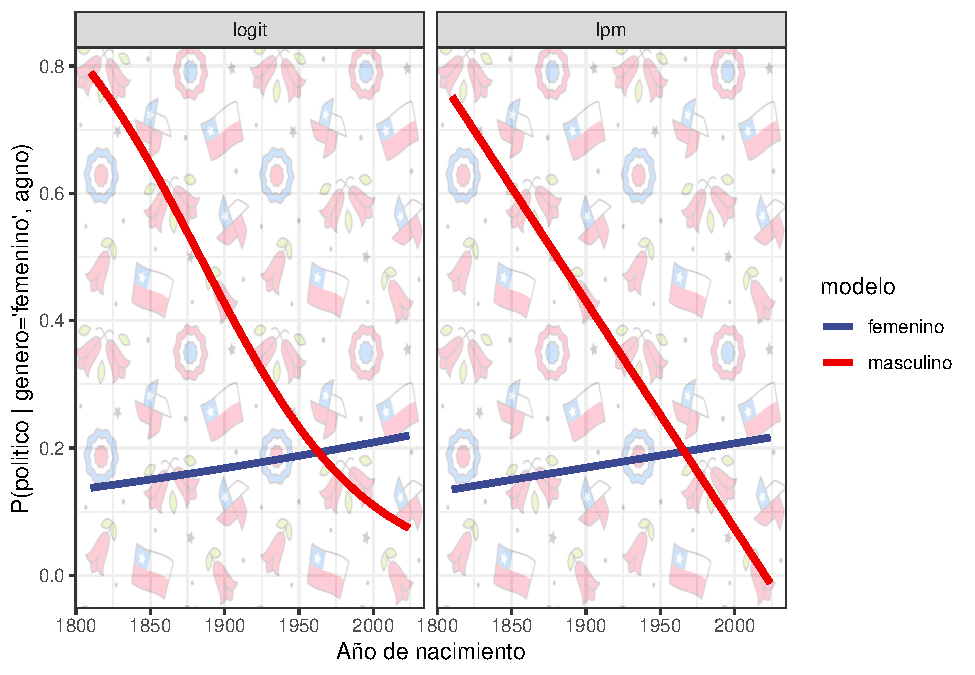
\includegraphics[width=0.8\linewidth]{01-trabajo-alaffert_files/figure-latex/unnamed-chunk-8-1}

\begin{enumerate}
\def\labelenumi{\arabic{enumi}.}
\setcounter{enumi}{2}
\tightlist
\item
  ¿En la regresión logística, cuál es el mayor efecto marginal posible de año de nacimiento sobre la probabilidad de ser político para hombres y mujeres? Compara con el respectivo efecto marginal en el LPM.
\end{enumerate}

El efecto marginal de año de nacimiento en el modelo logit estimado en el apartado anterior era de -0.00182 para mujeres y de -0.00234 para hombres. Para obtener el mayor efecto marginal posible, debemos evaluar el coeficiente en su valor máximo, es decir, cuando \(p\) = 0.5. Un atajo matemático para obtener el mismo resultado es dividir por 4 el efecto marginal obtenido:

Para mujeres:
\[
\text{Max marginal mujer} = \frac{-0.00182}{4} = -0.000455
\]

Para hombres:

\[
\text{Max marginal hombre} = \frac{-0.00234}{4} = -0.000585
\]

En el LPM del apartado I.2, el efecto marginal del año de nacimiento era de -0.003, el cual es constante o no tiene una diferenciación según género.

De este modo, el efecto marginal en el modelo logístico es más pequeño que en el LPM, pero depende de la probabilidad \(p\) y varía según los valores predichos de \(p\), mientras que en el LPM es constante.

\end{document}
